\setchapterpreamble[u]{\margintoc}
\chapter{单因素实验设计}
\labch{options}

以往在论述实验设计时,我们只交代了做一个随机区组或者用被试内可以带走无关变异这样一个事实,但这只是描述性的话,没有数据的前后对比无法让人真的信服随机区组和被试内设计的好处.所以,现在要从数据上看到$F$怎样更容易显著.

所谓$F$更容易显著无非就是$F$更大了($F=MSA/MSE$),想让$F$变大有两个手段,让处理效应($MSA$)变大,或者让误差效应($MSE$)变小,这件事情在前面已经介绍过.我说过心理学家感兴趣的那些现象往往都不太大\sidenote{也可以说是效应量(effect size)总是不太大},而且人为加大处理效应有时没有什么意义.从实验设计的角度上,减小误差才是关键.

\begin{marginfigure}
	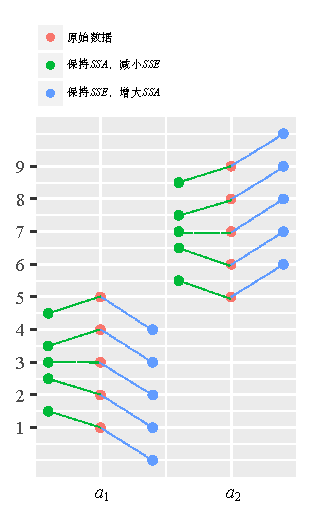
\includegraphics{SSA_SSE}
	\caption{红色是原始数据,蓝色代表组内误差不变,加大处理效应;绿色代表组间变异不变,改变组内误差}
	\labfig{SSA_SSE}
\end{marginfigure}

这就好比用天文望远镜观测外太空,我想发现人们不曾发现过的行星,我透过天文望远镜可以看到一些噪音——没有规律发亮的光点,但是那颗星星好像也在发光,我想鉴别这个星星是否真实存在,但是这件事情不是那么容易,因为星星发的光和噪音总是同时出现,故只有星星发出的光足够大,大到和周围的噪音是那么的与众不同,我再将这个星星是噪音有很大几率犯错,我才敢认定那是星星.我们清楚地知道,想要更加清楚地观察到星星无非有两种手段,其一是让星星在原有基础上多发电光;其二是让周围的噪音降低点.

方差分析模型中的$MSA$和$MSE$是相互独立的,它们俩可以独立地变化.随机误差指的是由随机因素导致数据在理想值周围随机晃动的偏差,它要是和处理不独立那就不能叫随机误差了.

\begin{kaobox}[frametitle=思考]
假定我们有一组分数,分别计算出$MSA$和$MSE$.

(1)我们可以改变$AS$\sidenote[*5][]{$AS$中A代表因素$A$的处理效应,$S$代表被试个体误差,具体是什么后面再说}分数,保持处理平均数恒定.即保持$MSA$不变而改变$MSE$.

(2)如果我们改变组平均数,处理组内分数关系不就,$MSA$会变化,而$MSE$不就.表明两个均方是独立变化的.

我们看一组数据

$a_1:1, 2, 3, 4, 5$

$a_2:5, 6, 7, 8, 9$

(1)调整原始数据,保持$SSA$不变,而$SSE$改变(减小$SSE$) (通常加大处理效应实现)

(2)调整原始数据,改变$SSA$不变(增大$SSA$),而$SSE$不变
\end{kaobox}



我直接给出我的思路,\reffig{SSA_SSE}中红色是原始数据,它有两个水平,$a_1$的各个值围绕其均值3波动,$a_2$的各个值围绕其均值7波动.

绿色是我写的符合(1)的一组数据,可以看到红色数据$a_1$处理的每个数据都围绕着3波动,现在绿色的值在$a_1$内还是围绕3波动,但是数据间的距离更短了,它们显得更加紧密.虽然从组内均值上来看(3和7)两组数据的平均值之差不变,但是由于$a_1$的数据更集中于3,$a_2$的数据更集中于7,故实际上这样两组间的差异其实增大了.

蓝色是我写的符合(2)的一组数据,可以看到数据间的紧密程度不变,$a_1$整体向下移动,$a_2$整体向上移动,这样组间的差距被拉大.

原始数据方差分析结果是.

\begin{table}[h]
	\centering
	\caption{原始数据方差分析}
	\labtab{RAW_ANOVA}
	{
		\begin{tabular}{cccccc}
			\toprule
			变异来源 & $SS$ & $df$ & $MS$ & $F$ & $p$  \\
			\cmidrule[0.4pt]{1-6}
			组间变异 & 40.000 & 1.000 & 40.000 & 16.000 & 0.004  \\
			组内变异 & 20.000 & 8.000 & 2.500 &  &    \\
			\bottomrule
			% \addlinespace[1ex]
			% \multicolumn{6}{p{0.5\linewidth}}{\textit{Note.} Type I Sum of Squares} \\
		\end{tabular}
	}
\end{table}

\begin{margintable}
    \caption{保持$SSA$不变,减小$SSE$}
    \labtab{lower_SSE}
    \raggedright
    \begin{tabular}{cccccc}
        \hline
        $a_1$ & 1.5 & 2.5 & 3 & 3.5 & 4.5\\
        $a_2$ & 5.5 & 6.5 & 7 & 7.5 & 8.5\\
        \hline
    \end{tabular}
\end{margintable}

绿色数据见\vreftab{lower_SSE}.


其方差分析结果是,可以看到相比\vreftab{RAW_ANOVA}中的数据,处理效应没变,误差效应减小了,$F$值变大,$p$值减小.

\begin{table}[h]
	\centering
	\caption{绿色数据方差分析}
	\label{tab:aNOVA-Score}
	{
		\begin{tabular}{cccccc}
			\toprule
			变异来源 & $SS$ & $df$ & $MS$ & $F$ & $p$  \\
			\cmidrule[0.4pt]{1-6}
			组间变异 & 40.000 & 1.000 & 40.000 & 32.000 & $<$ .001  \\
			组内变异 & 10.000 & 8.000 & 1.250 &  &    \\
			\bottomrule
			% \addlinespace[1ex]
			% \multicolumn{6}{p{0.5\linewidth}}{\textit{Note.} Type III Sum of Squares} \\
		\end{tabular}
	}
\end{table}

\begin{margintable}
    \caption{保持$SSE$不变,增大$SSA$}
    \labtab{UPPER_SSA}
    \raggedright
    \begin{tabular}{cccccc}
        \hline
        $a_1$ & 1 & 1 & 2 & 3 & 4\\
        $a_2$ & 6 & 7 & 8 & 8 & 10\\
        \hline
    \end{tabular}
\end{margintable}

蓝色数据见\vreftab{UPPER_SSA}.

其方差分析结果是,可以看到相比\vreftab{RAW_ANOVA}中的数据,处理效应变大,组内误差减没变,$F$值变大,$p$值减小.

\begin{table}[h]
	\centering
	\caption{蓝色数据方差分析}
	\label{tab:aNOVA-Score}
	{
		\begin{tabular}{cccccc}
			\toprule
			变异来源 & $SS$ & $df$ & $MS$ & $F$ & $p$  \\
			\cmidrule[0.4pt]{1-6}
			组间变异 & 90.000 & 1.000 & 90.000 & 36.000 & $<$ .001  \\
			组内变异 & 20.000 & 8.000 & 2.500 &  &    \\
			\bottomrule
			% \addlinespace[1ex]
			% \multicolumn{6}{p{0.5\linewidth}}{\textit{Note.} Type III Sum of Squares} \\
		\end{tabular}
	}
\end{table}




\section{单因素完全随机实验设计}
\subsection{单因素完全随机设计的基本特点}

完全随机设计的假定是,由于被试是从总体中随机选取,处理也是随机分配给被试,那么被试间的差异也是随机、在统计上无差异的.

\begin{margintable}
	\centering
	\caption{单因素完全随机实验设计中被试的分配}
	\labtab{one_way_ANOVA_data}
	{
		\begin{tabular}{cccc}
			\toprule
			$a_1$ & $a_2$ & $a_3$ & $a_4$ \\
			\cmidrule[0.4pt]{1-4}
			$S_1$ & $S_2$ & $S_3$ & $S_4$ \\
			$S_5$ & $S_6$ & $S_7$ & $S_8$ \\
			$S_9$ & $S_{10}$ & $S_{11}$ & $S_{12}$ \\
			$S_{13}$ & $S_{14}$ & $S_{15}$ & $S_{16}$ \\
			\bottomrule
			% \addlinespace[1ex]
			% \multicolumn{6}{p{0.5\linewidth}}{\textit{Note.} Type III Sum of Squares} \\
		\end{tabular}
	}
\end{margintable}

单因素完全随机设计中分配被试的图解例子如\vreftab{one_way_ANOVA_data},
个因素$A$有4个水平,每个处理下有4个被试.完全随机设计是一种被试间设计,这意味着每一个被试只接受一种处理或处理的组合
\sidenote[*-5][]{处理的组合是多因素实验中会遇到的,后面遇到了再说}
,故对于本例而言需要16个被试.

对按下来要描述的模型的字母进行一下简要的说明:

(1)假设因素$A$有$p$个水平,用$\alpha _j$表示其第$j$个水平($1 \leq j \leq p$),也就是说$A$的水平分别是$\alpha _1,...,\alpha _j,..., \alpha _p$,

(2)$p$个处理下的被试数都相等,均为$n$个,用$i$表示每个处理下第$i$个被试($1 \leq i \leq n$)

(3)假设被试在没有施加处理的时候,无限次实验结果的平均数是$\mu$.该值是个理想值,其实意思是被试测量值在理论上的基线,不过这么说只是表达了概念.虽然说明了更加明确的定义不过可以充分的感受到,这个理论基线值是无法获得的,毕竟无限次是个极限,不是一个具体的数,所以$\mu$是个理论值.

(4)假设实验中的误差是$\varepsilon _{i\left(j\right)}$
\sidenote{关于为什么它的下标是带括号的现在不便解释.}
,其平均数为0,方差为$\sigma _e^2$,我们进一步假设它服从正态分布

(4)观察值$Y_{ij}$指第$j$个处理水平下,第$i$个被试的观测值

后现的章节因素多了会加入一些新字母和下标,和上述符号已经没有本质区别,故以后我不打算再介绍新符号了.

单因素完全随机设计的原假说是:多个处理水平上的总体平均数相等,即
$$
H_0: \mu _{.1}=\mu _{.2}=...=\mu _{.p}
$$

或处理效应等于为0,即
$$
\alpha _j=0
$$


单因素完全随机实验设计模型
\begin{equation}
    Y_{ij}=\mu +\alpha _j+\varepsilon _{i\left( j \right)}
\end{equation}
其中:

\begin{table}[h]
	\centering
	%\caption{单因素完全随机实验设计中被试的分配}
	%\labtab{one_way_ANOVA_data}
	{
		\begin{tabular}{lcl}
			$Y_{ij}$ & —— & 被试$i$在处理水平$j$上的分数 \\
			$\mu$ & —— & 总体平均数 \\
			$\alpha _j$ & —— & 水平$j$的处理效应 \\
			$\varepsilon_{i \left( j \right)}$ & —— & 误差效应 \\
		\end{tabular}
	}
\end{table}


\subsection{单因素完全随机实验设计与计算举例}

\subsubsection{研究的问题}
我想研究文章的生字密度对学生阅读理解的影响.我的假设是:阅读理解随着文章中生字密度的增加而下降。因此,该实验有一个自变量——生字密度,通过研究前人文献我感兴趣的是四种生字密度
(1)$5:1(a_1)$
(2)$10:1(a_2)$
(3)$15:1(a_3)$
(4)$20:1(a_4$
因变量是被试的阅读理解分数。实施实验时,我将32名被试随机分成四组,每组被试阅读一种生字密度的文章,并回答阅读理解测验中有关文章内容的问题。这是一个典型的单因素完全随机设计。虽然我不再检验实验中其他因素的影响,但实际上存在着诸多对因变量影响的无关变量,比如文章的长度、文章的主题熟悉性、文章类型等,还有被试的年龄、受教育程度、阅读能力等。这时,控制无关变量可做的工作之一是在选取四篇文章时,使它们在除生字密度以外的其他方面尽量匹配。

\subsubsection{新的计算模型的引入以及数据的计算}
我将引入一种新的计算模式,这种模式主要是为了手算.为了理解愿意,我们必须手算一次每种实验设计的简单数据,但是用统计教材上的算法根本无法实现一个较为精确的估算,其原因是,和方的计算公式选用:

$$
    SS =
        \sum\limits_{i=1}^{n}
        \left( 
            X_i -\bar{X} 
        \right)^2
$$

式子中$\bar{X}$很大可能是小数,且可能是循环小数,所以每次相减都会四舍五入,然后平方后进一步放大误差,这样算到最后误差不断累记.此时要提出的思路是,最后一步再做除法.

\begin{description}
\item[1.计算表] 
\begin{margintable}
	\centering
	\caption{单因素完全随机实验的$AS$表}
	\label{one_way_ANOVA_AS_TAB}
	{
		\begin{tabular}{cccccc}
			\toprule
    			     & $a_1$ &  $a_2$ &  $a_3$ &  $a_4$ & \\
                              & \cellcolor[rgb]{ .851,  .851,  .851}3 & \cellcolor[rgb]{ .851,  .851,  .851}4 & \cellcolor[rgb]{ .851,  .851,  .851}8 & \cellcolor[rgb]{ .851,  .851,  .851}9 &  \\
                              & \cellcolor[rgb]{ .851,  .851,  .851}6 & \cellcolor[rgb]{ .851,  .851,  .851}6 & \cellcolor[rgb]{ .851,  .851,  .851}9 & \cellcolor[rgb]{ .851,  .851,  .851}8 &  \\
                              & \cellcolor[rgb]{ .851,  .851,  .851}4 & \cellcolor[rgb]{ .851,  .851,  .851}4 & \cellcolor[rgb]{ .851,  .851,  .851}8 & \cellcolor[rgb]{ .851,  .851,  .851}8 &  \\
                              & \cellcolor[rgb]{ .851,  .851,  .851}3 & \cellcolor[rgb]{ .851,  .851,  .851}2 & \cellcolor[rgb]{ .851,  .851,  .851}7 & \cellcolor[rgb]{ .851,  .851,  .851}7 &  \\
                              & \cellcolor[rgb]{ .851,  .851,  .851}5 & \cellcolor[rgb]{ .851,  .851,  .851}4 & \cellcolor[rgb]{ .851,  .851,  .851}5 & \cellcolor[rgb]{ .851,  .851,  .851}12 &  \\
                              & \cellcolor[rgb]{ .851,  .851,  .851}7 & \cellcolor[rgb]{ .851,  .851,  .851}5 & \cellcolor[rgb]{ .851,  .851,  .851}6 & \cellcolor[rgb]{ .851,  .851,  .851}13 &  \\
                              & \cellcolor[rgb]{ .851,  .851,  .851}5 & \cellcolor[rgb]{ .851,  .851,  .851}3 & \cellcolor[rgb]{ .851,  .851,  .851}7 & \cellcolor[rgb]{ .851,  .851,  .851}12 &  \\
                              & \cellcolor[rgb]{ .851,  .851,  .851}2 & \cellcolor[rgb]{ .851,  .851,  .851}3 & \cellcolor[rgb]{ .851,  .851,  .851}6 & \cellcolor[rgb]{ .851,  .851,  .851}11 &  \\
                        总     & \cellcolor[rgb]{ .886,  .937,  .855}35 & \cellcolor[rgb]{ .886,  .937,  .855}31 & \cellcolor[rgb]{ .886,  .937,  .855}56 & \cellcolor[rgb]{ .886,  .937,  .855}80 & \cellcolor[rgb]{ .867,  .922,  .969}202 \\

			\bottomrule
		\end{tabular}
	}
\end{margintable}

\item[2.各种基本量的计算]
    \[
        \sum\limits_{i=1}^{n} \sum\limits_{j=1}^{p}Y_{ij} = 3+6+4+...=202.000\\
    \]
    \begin{align*}
        %----------------------------------------------------------
        %[Y]
            \frac{
                \left(
        	\sum\limits_{i=1}^{n} \sum\limits_{j=1}^{p}Y_{ij}
                \right)^2}
            {np}=& \colorbox[rgb]{ .867,  .922,  .969}{$[Y]$} = 
            \frac{
                \left(
        	    202
                \right)^2}
                {
                    \left(
        	           8
                    \right)^2
                    \left(
                        4
                    \right)^2
                }&=1275.125\\
        %----------------------------------------------------------
        %[AS]
            \sum\limits_{i=1}^{n} \sum\limits_{j=1}^{p}Y_{ij}^2=
            & \colorbox[rgb]{ .851,  .851,  .851}{$[AS]$} = 
            \left(
            	3
            \right)^2 +
            \left(
            	6
            \right)^2    +... &=1544.000\\
        %----------------------------------------------------------
        %[A]    
            \sum\limits_{i=1}^{n}
            \frac
                {\left(
	            \sum\limits_{j=1}^{p}Y_{ij}
                \right)^2}
                {n}=
            &\colorbox[rgb]{ .886,  .937,  .855}{$[A]$}=
            \frac{\left(35\right)^2}{8}+\frac{\left(31\right)^2}{8}+...&=1465.250            
    \end{align*}
    
\item[3.平方和分解与计算]
    \begin{align*}
        SS_{\text{总}} & = SS_{\text{组间}}+SS_{\text{组内}}\\
        SS_{\text{总}} & = [AS]-[Y]=268.875\\
        SS_{\text{组间}} & = SSA=[A]-[Y]=190.125\\
        SS_{\text{组内}} & = SSE=SS_{\text{总}}-SS_{\text{组间}}=78.750
    \end{align*}
    
\item[4.方差分析表及结果的解释]

\begin{table}[h]
	\centering
	\caption{单因素完全随机实验的方差分析表}
	\label{one_way_ANOVA_Tab}
	{
		\begin{tabular}{cccccc}
			\toprule
			变异源 & $SS$ & $df$ & $MS$ & $F$ & $p$  \\
			\cmidrule[0.4pt]{1-6}
			组间(生字密度) & 190.125 & $p-1=3$ & 63.375 & 22.533 & $<$ .001  \\
			组内(个体误差) & 78.750 & $p(n-1)=28$ & 2.813 &  &    \\
			\cmidrule[0.4pt]{1-6}
			总计 & 268.875 & $np-1=31$ & & &\\
			\bottomrule
			% \addlinespace[1ex]
			% \multicolumn{6}{p{0.5\linewidth}}{\textit{Note.} Type III Sum of Squares} \\
		\end{tabular}
	}
\end{table}

方差分析结果表明,生字密度的效应是显著的($F(3,28)=22.53(p<0.01)$),生字不同的文章对学生的学生阅读理解有显著的影响。从阅读理解的四种生字密度文章的平均数可以初步看出

\item[5.平方和与自由度分解图]
\begin{equation}
    SS_{\text{总}} \begin{cases}
    SS_{\text{组间}}\\
    SS_{\text{组内}}
\end{cases}
\end{equation}
\[
    SS_\text{总} \quad df=np-1=31\\
    SS_{\text{组间}} \quad df=p-1=3\\
    SS_{\text{组内}} \quad df=p(n-1)=28
\]
\item[6.对平方和分解与计算的一些解释]
\end{description}










\section{单因素随机区组实验设计}

\section{单因素拉丁方实验设计}

\section{单因素被试内实验设计}